%\documentclass[14pt]{beamer}
\documentclass{beamer}

\usepackage{listings}
\usepackage{cpp}

\usetheme{Copenhagen}
% \usetheme{Boadilla}
% \usecolortheme{beaver}
\setbeamercolor{alerted text}{fg=orange}
\setbeamercolor{background canvas}{bg=white}
\setbeamercolor{block body alerted}{bg=normal text.bg!90!black}
\setbeamercolor{block body}{bg=normal text.bg!90!black}
\setbeamercolor{block body example}{bg=normal text.bg!90!black}
\setbeamercolor{block title alerted}{use={normal text,alerted text},fg=alerted text.fg!75!normal text.fg,bg=normal text.bg!75!black}
\setbeamercolor{block title}{bg=blue}
\setbeamercolor{block title example}{use={normal text,example text},fg=example text.fg!75!normal text.fg,bg=normal text.bg!75!black}
\setbeamercolor{fine separation line}{}
\setbeamercolor{frametitle}{fg=white}
\setbeamercolor{item projected}{fg=white}
\setbeamercolor{normal text}{bg=white,fg=black}
\setbeamercolor{palette sidebar primary}{use=normal text,fg=normal text.fg}
\setbeamercolor{palette sidebar quaternary}{use=structure,fg=structure.fg}
\setbeamercolor{palette sidebar secondary}{use=structure,fg=structure.fg}
\setbeamercolor{palette sidebar tertiary}{use=normal text,fg=normal text.fg}
\setbeamercolor{section in sidebar}{fg=brown}
\setbeamercolor{section in sidebar shaded}{fg=grey}
\setbeamercolor{separation line}{}
\setbeamercolor{sidebar}{bg=red}
\setbeamercolor{sidebar}{parent=palette primary}

\setbeamercolor{structure}{bg=black, fg=white!30!blue!70!green}

\setbeamercolor{subsection in sidebar}{fg=brown}
\setbeamercolor{subsection in sidebar shaded}{fg=grey}
\setbeamercolor{title}{fg=white}
\setbeamercolor{titlelike}{fg=white}

% Szép kék
% \setbeamercolor{structure}{bg=black, fg=white!10!green!40!blue}

\frenchspacing

% Language packages
\usepackage[utf8]{inputenc}
\usepackage[T1]{fontenc}
\usepackage[magyar]{babel}

% AMS
\usepackage{amssymb,amsmath}

% Graphic packages
\usepackage{graphicx}

% Syntax highlighting
\usepackage{listings}

\usepackage{tikz}

\usepackage{hyperref}

% ==============
\begin{document}
% ==============

\title[Alternatív grafikus megjelenítési módok]{Alternatív grafikus megjelenítési módok}
\author[Vécsi Ádám]{\textbf{Vécsi Ádám}}
\institute[]{Miskolci Egyetem}
% \date{ME, 2014. november 6.}
\date{Miskolci Egyetem, 2018. június 12.}

% --------------------
\frame{\titlepage}

% --------------------
\begin{frame}[fragile]
\frametitle{Művészi szűrők}

Alkalmazási területek
\begin{itemize}
\item Közösségi alkalmazások
\item Webkamera- és mobil alkalmazások
\item Filmek, játékok
\end{itemize}

\bigskip

\begin{center}
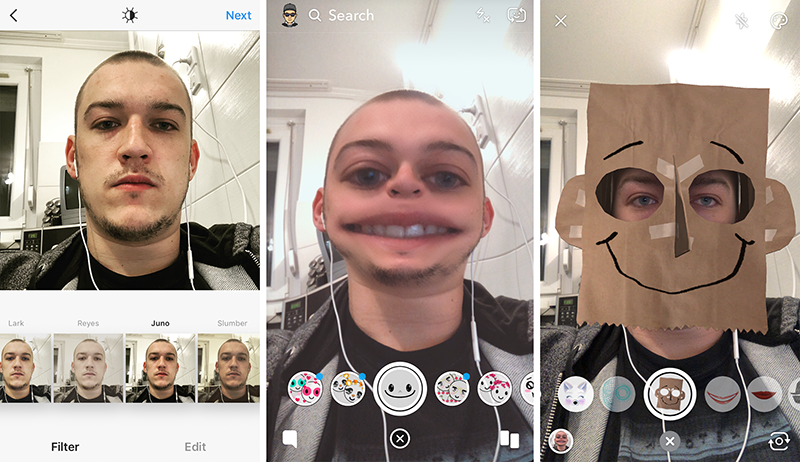
\includegraphics[scale=0.25]{kepek/instasnapmess.png}
\end{center}

\end{frame}

% --------------------
\begin{frame}[fragile]
\frametitle{További példák}

\begin{center}

\includegraphics[scale=0.1]{kepek/prismawebcam.jpg}
\end{center}

\begin{center}
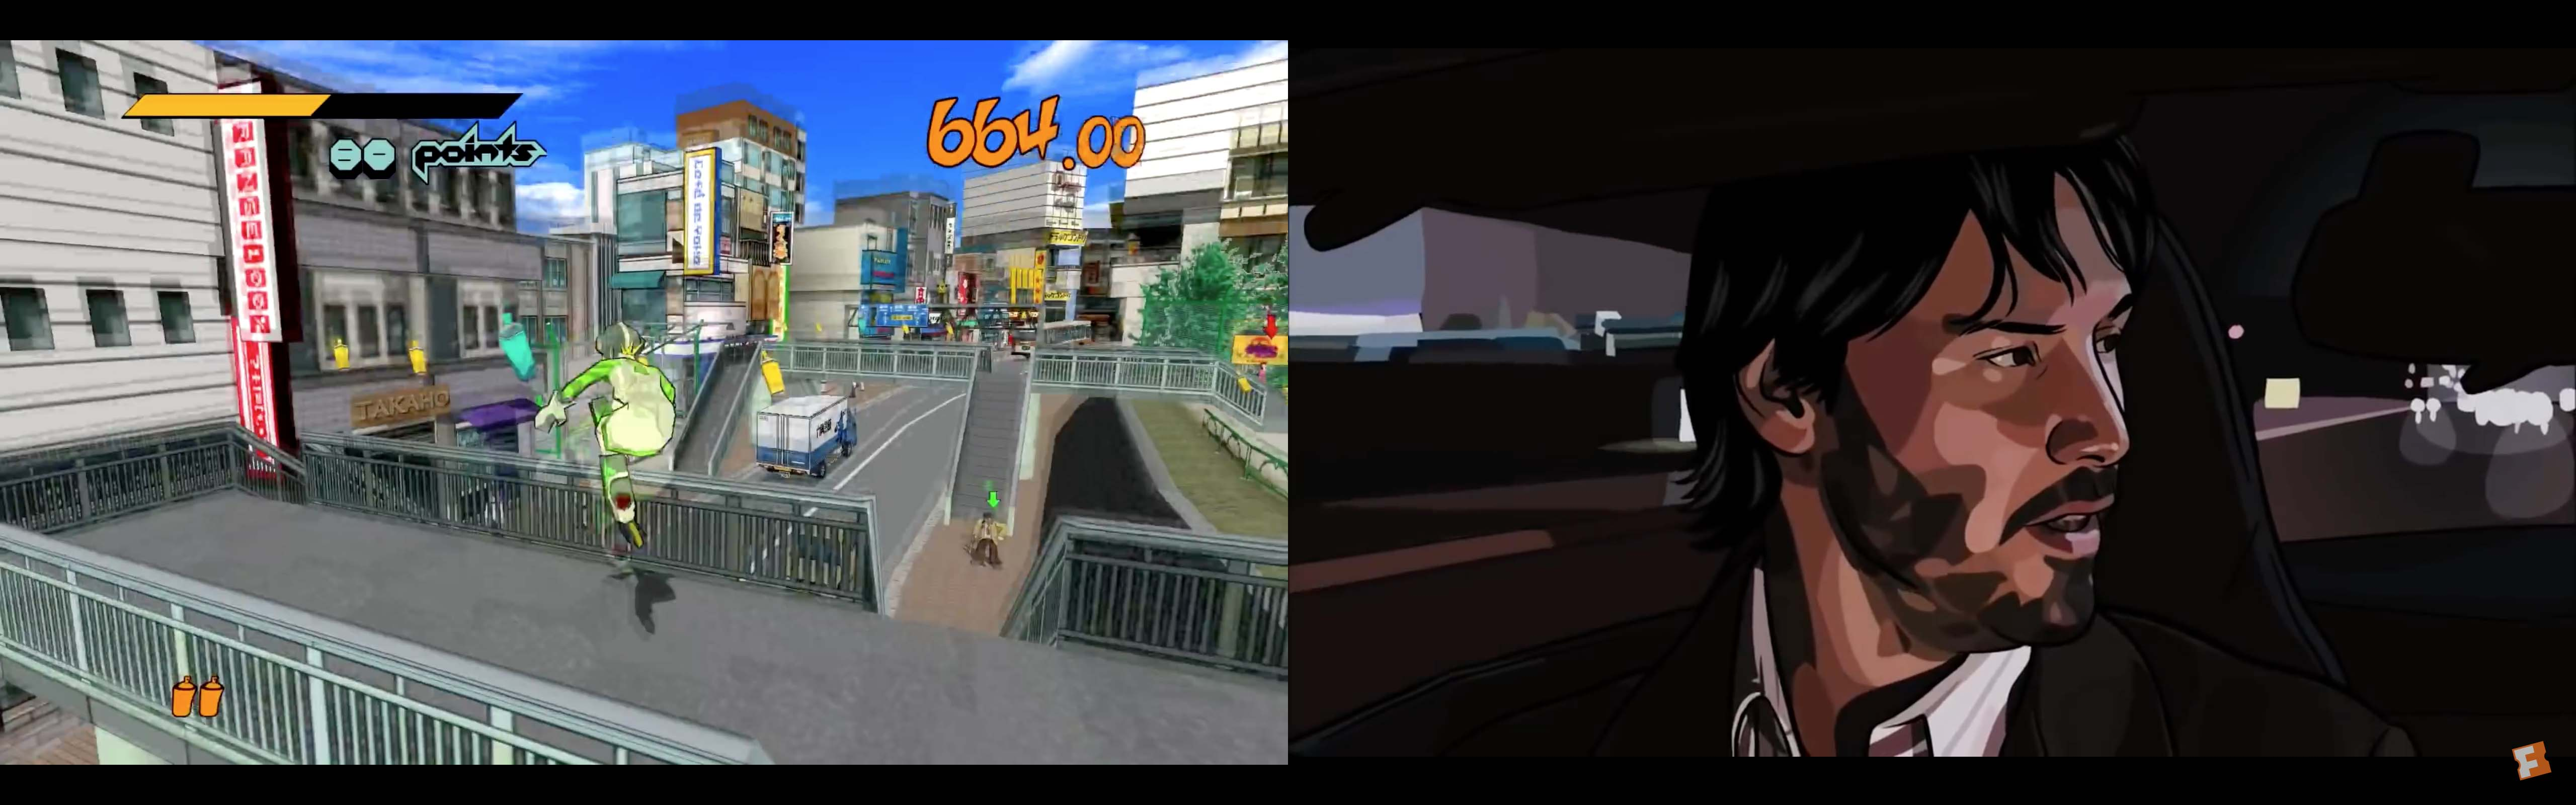
\includegraphics[scale=0.1]{kepek/jatekfilm.jpg}
\end{center}

\end{frame}

% --------------------
\begin{frame}[fragile]
\frametitle{Matematikai eszközök}

\textbf{Zajok szűrése, elmosás}

\begin{itemize}
\item Átlagoló szűrő
\item Gauss szűrő
\item Medián szűrő
\item Kétoldali szűrő
\end{itemize}

\bigskip

\textbf{Élkiemelés}

\begin{itemize}
\item
Sobel éldetektálás
$$
G_x =
\begin{bmatrix}
-1&0  &1 \\ 
-2&0  &2 \\ 
-1&0  &1 
\end{bmatrix},
\qquad
G_y =
\begin{bmatrix}
-1&-2  &-1 \\ 
0&0  &0 \\ 
1&2  &1 
\end{bmatrix}.
$$
\item Laplace éldetektálás
\item Canny éldetektálás
\end{itemize}

\end{frame}

% --------------------
\begin{frame}[fragile]
\frametitle{Matematikai eszközök}

\textbf{Szegmentálás}

\begin{itemize}
\item Mean shift algoritmus
\end{itemize}

\bigskip

\textbf{Küszöbölés}

A cél a megfelelő globális és lokális küszöbértékek meghatározása.

\begin{itemize}
\item Izodata algoritmus (Yanni)
\item Otsu algoritmus
\item Niblack algoritmus
\end{itemize}

\end{frame}

% --------------------
\begin{frame}[fragile]
\frametitle{Szűrő algoritmusok}

Saját készítésű művészi szűrők

\begin{itemize}
\item Cartoon-style filter
\item Pencil sketch filter
\item Cartoon filter
\item Aquarelle-style filter
\end{itemize}

\end{frame}

% --------------------
\begin{frame}[fragile]
\frametitle{Cartoon-style filter}

\end{frame}

% --------------------
\begin{frame}[fragile]
\frametitle{Pencil sketch filter}

\end{frame}

% --------------------
\begin{frame}[fragile]
\frametitle{Cartoon filter}

\end{frame}


% --------------------
\begin{frame}[fragile]
\frametitle{Aquarelle-style filter}

\end{frame}

% --------------------
\begin{frame}[fragile]
\frametitle{Implementáció}

\textbf{OpenCV}

\begin{itemize}
\item Beépített művészi szűrők áttekintése
\item Mind a 4 szűrőnek külön C++ projekt
\end{itemize}

\medskip

\textbf{Megoldandó feladatok}

\begin{itemize}
\item Képek betöltése, ablak megjelenítése
\item Elmosásos szűrők
\end{itemize}

\begin{cpp}
GaussianBlur(source, gauss, ksize, sigmaX, sigmaY);
medianBlur(source, median, kernel_size);
\end{cpp}

\begin{itemize}
\item Küszöbölés
\end{itemize}

\begin{cpp}
threshold(src, res, thr, maxval, THRESH_BINARY_INV);
\end{cpp}

\end{frame}


% --------------------
\begin{frame}[fragile]
\frametitle{Tesztek, eredmények}

\begin{itemize}
\item Elsősorban futási időre vonatkozóan
\item Konfiguráció: MacBook Pro, Intel Core i5, 8GB RAM, Intel Iris
\item Költséges ablaklétrehozási, képbetöltési idők
\item Jelentős számítási idő a konvolúciós műveleteknél
\end{itemize}

\end{frame}

% --------------------
\begin{frame}[fragile]
\frametitle{Cartoon-style filter számítási ideje}

\end{frame}

% --------------------
\begin{frame}[fragile]
\frametitle{Pencil sketch számítási ideje}

\end{frame}

% --------------------
\begin{frame}[fragile]
\frametitle{Összegzés}

\end{frame}

% --------------------
\begin{frame}[fragile]
\frametitle{Hivatkozások}

1

12

15

16

17

\end{frame}

% --------------------
\begin{frame}[fragile]
    \frametitle{\ }

\begin{center}
\Large \textbf{Köszönöm szépen a figyelmet!}
\end{center}

\end{frame}


\end{document}
